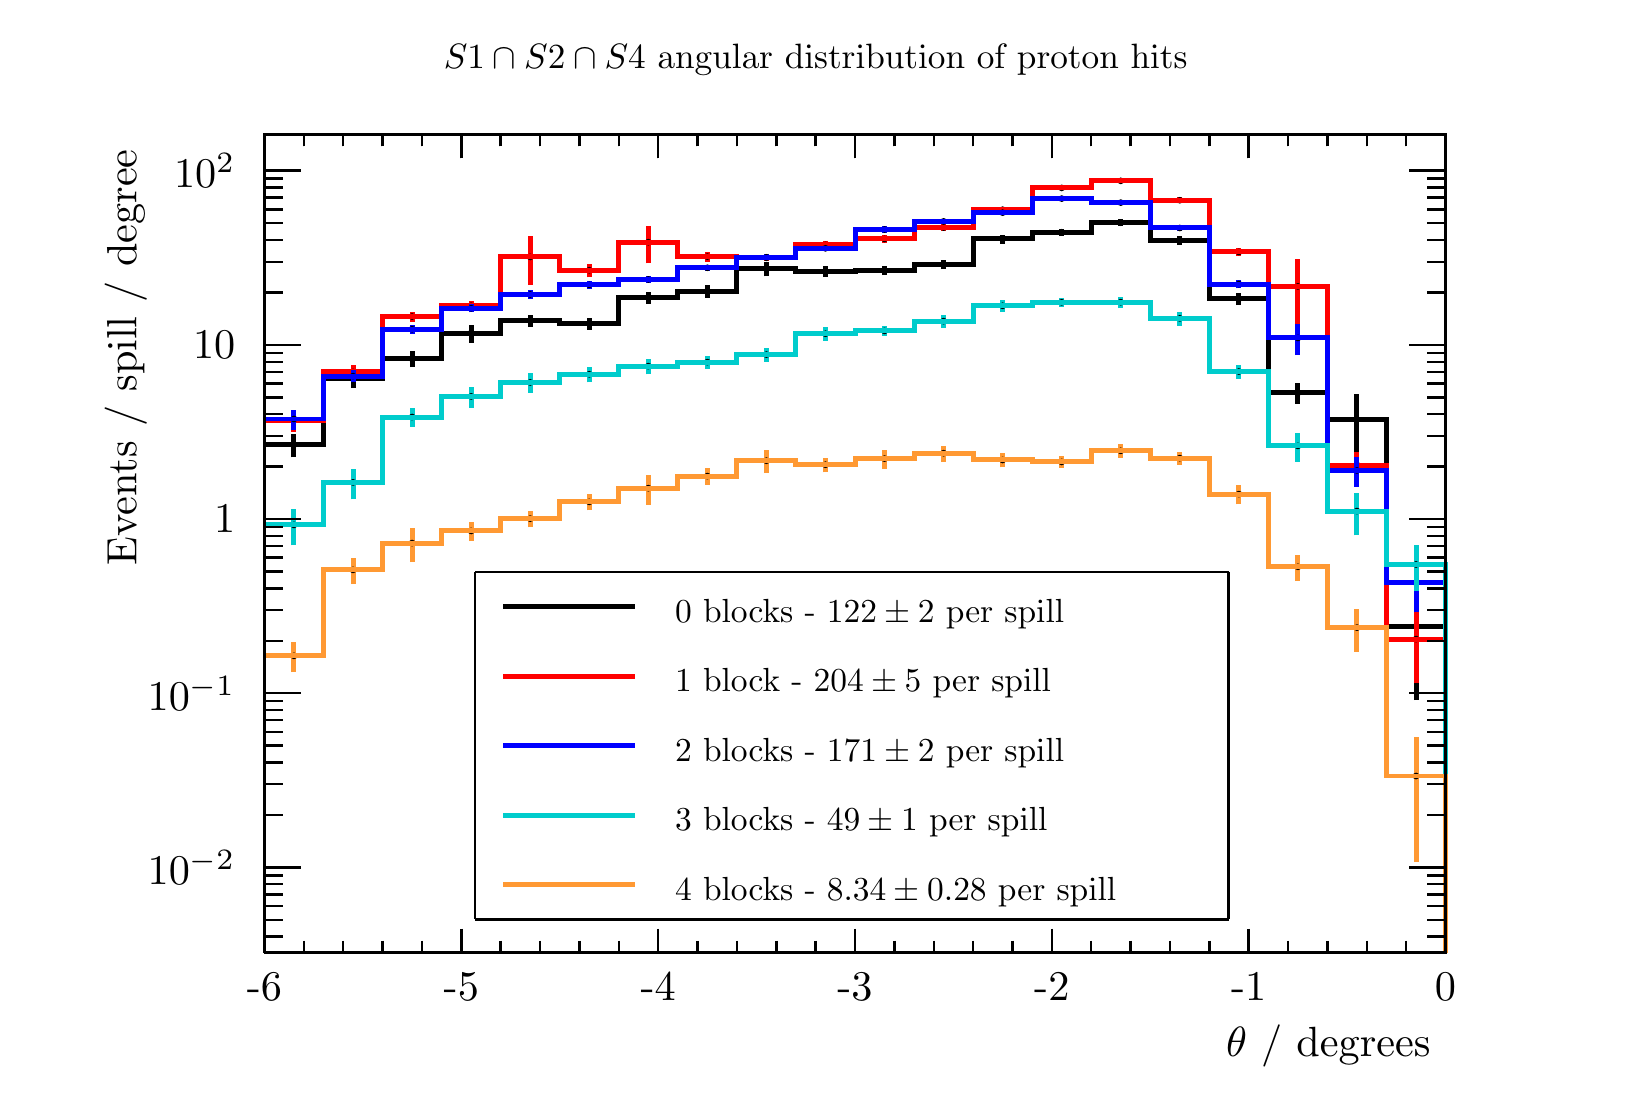
\begin{tikzpicture}
\pgfdeclareplotmark{cross} {
\pgfpathmoveto{\pgfpoint{-0.3\pgfplotmarksize}{\pgfplotmarksize}}
\pgfpathlineto{\pgfpoint{+0.3\pgfplotmarksize}{\pgfplotmarksize}}
\pgfpathlineto{\pgfpoint{+0.3\pgfplotmarksize}{0.3\pgfplotmarksize}}
\pgfpathlineto{\pgfpoint{+1\pgfplotmarksize}{0.3\pgfplotmarksize}}
\pgfpathlineto{\pgfpoint{+1\pgfplotmarksize}{-0.3\pgfplotmarksize}}
\pgfpathlineto{\pgfpoint{+0.3\pgfplotmarksize}{-0.3\pgfplotmarksize}}
\pgfpathlineto{\pgfpoint{+0.3\pgfplotmarksize}{-1.\pgfplotmarksize}}
\pgfpathlineto{\pgfpoint{-0.3\pgfplotmarksize}{-1.\pgfplotmarksize}}
\pgfpathlineto{\pgfpoint{-0.3\pgfplotmarksize}{-0.3\pgfplotmarksize}}
\pgfpathlineto{\pgfpoint{-1.\pgfplotmarksize}{-0.3\pgfplotmarksize}}
\pgfpathlineto{\pgfpoint{-1.\pgfplotmarksize}{0.3\pgfplotmarksize}}
\pgfpathlineto{\pgfpoint{-0.3\pgfplotmarksize}{0.3\pgfplotmarksize}}
\pgfpathclose
\pgfusepathqstroke
}
\pgfdeclareplotmark{cross*} {
\pgfpathmoveto{\pgfpoint{-0.3\pgfplotmarksize}{\pgfplotmarksize}}
\pgfpathlineto{\pgfpoint{+0.3\pgfplotmarksize}{\pgfplotmarksize}}
\pgfpathlineto{\pgfpoint{+0.3\pgfplotmarksize}{0.3\pgfplotmarksize}}
\pgfpathlineto{\pgfpoint{+1\pgfplotmarksize}{0.3\pgfplotmarksize}}
\pgfpathlineto{\pgfpoint{+1\pgfplotmarksize}{-0.3\pgfplotmarksize}}
\pgfpathlineto{\pgfpoint{+0.3\pgfplotmarksize}{-0.3\pgfplotmarksize}}
\pgfpathlineto{\pgfpoint{+0.3\pgfplotmarksize}{-1.\pgfplotmarksize}}
\pgfpathlineto{\pgfpoint{-0.3\pgfplotmarksize}{-1.\pgfplotmarksize}}
\pgfpathlineto{\pgfpoint{-0.3\pgfplotmarksize}{-0.3\pgfplotmarksize}}
\pgfpathlineto{\pgfpoint{-1.\pgfplotmarksize}{-0.3\pgfplotmarksize}}
\pgfpathlineto{\pgfpoint{-1.\pgfplotmarksize}{0.3\pgfplotmarksize}}
\pgfpathlineto{\pgfpoint{-0.3\pgfplotmarksize}{0.3\pgfplotmarksize}}
\pgfpathclose
\pgfusepathqfillstroke
}
\pgfdeclareplotmark{newstar} {
\pgfpathmoveto{\pgfqpoint{0pt}{\pgfplotmarksize}}
\pgfpathlineto{\pgfqpointpolar{44}{0.5\pgfplotmarksize}}
\pgfpathlineto{\pgfqpointpolar{18}{\pgfplotmarksize}}
\pgfpathlineto{\pgfqpointpolar{-20}{0.5\pgfplotmarksize}}
\pgfpathlineto{\pgfqpointpolar{-54}{\pgfplotmarksize}}
\pgfpathlineto{\pgfqpointpolar{-90}{0.5\pgfplotmarksize}}
\pgfpathlineto{\pgfqpointpolar{234}{\pgfplotmarksize}}
\pgfpathlineto{\pgfqpointpolar{198}{0.5\pgfplotmarksize}}
\pgfpathlineto{\pgfqpointpolar{162}{\pgfplotmarksize}}
\pgfpathlineto{\pgfqpointpolar{134}{0.5\pgfplotmarksize}}
\pgfpathclose
\pgfusepathqstroke
}
\pgfdeclareplotmark{newstar*} {
\pgfpathmoveto{\pgfqpoint{0pt}{\pgfplotmarksize}}
\pgfpathlineto{\pgfqpointpolar{44}{0.5\pgfplotmarksize}}
\pgfpathlineto{\pgfqpointpolar{18}{\pgfplotmarksize}}
\pgfpathlineto{\pgfqpointpolar{-20}{0.5\pgfplotmarksize}}
\pgfpathlineto{\pgfqpointpolar{-54}{\pgfplotmarksize}}
\pgfpathlineto{\pgfqpointpolar{-90}{0.5\pgfplotmarksize}}
\pgfpathlineto{\pgfqpointpolar{234}{\pgfplotmarksize}}
\pgfpathlineto{\pgfqpointpolar{198}{0.5\pgfplotmarksize}}
\pgfpathlineto{\pgfqpointpolar{162}{\pgfplotmarksize}}
\pgfpathlineto{\pgfqpointpolar{134}{0.5\pgfplotmarksize}}
\pgfpathclose
\pgfusepathqfillstroke
}
\definecolor{c}{rgb}{1,1,1};
\draw [color=c, fill=c] (0,0) rectangle (20,13.4957);
\draw [color=c, fill=c] (3,1.75444) rectangle (18,12.1461);
\definecolor{c}{rgb}{0,0,0};
\draw [c,line width=0.9] (3,1.75444) -- (3,12.1461) -- (18,12.1461) -- (18,1.75444) -- (3,1.75444);
\definecolor{c}{rgb}{1,1,1};
\draw [color=c, fill=c] (3,1.75444) rectangle (18,12.1461);
\definecolor{c}{rgb}{0,0,0};
\draw [c,line width=0.9] (3,1.75444) -- (3,12.1461) -- (18,12.1461) -- (18,1.75444) -- (3,1.75444);
\draw [c,line width=0.9] (3,1.75444) -- (3.75,1.75444) -- (3.75,1.75444) -- (4.5,1.75444) -- (4.5,1.75444) -- (5.25,1.75444) -- (5.25,1.75444) -- (6,1.75444) -- (6,1.75444) -- (6.75,1.75444) -- (6.75,1.75444) -- (7.5,1.75444) -- (7.5,1.75444) --
 (8.25,1.75444) -- (8.25,1.75444) -- (9,1.75444) -- (9,1.75444) -- (9.75,1.75444) -- (9.75,1.75444) -- (10.5,1.75444) -- (10.5,1.75444) -- (11.25,1.75444) -- (11.25,1.75444) -- (12,1.75444) -- (12,1.75444) -- (12.75,1.75444) -- (12.75,1.75444) --
 (13.5,1.75444) -- (13.5,1.75444) -- (14.25,1.75444) -- (14.25,1.75444) -- (15,1.75444) -- (15,1.75444) -- (15.75,1.75444) -- (15.75,1.75444) -- (16.5,1.75444) -- (16.5,1.75444) -- (17.25,1.75444) -- (17.25,1.75444) -- (18,1.75444) -- (18,1.75444);
\draw [c,line width=0.9] (3,1.75444) -- (18,1.75444);
\draw [c,line width=0.9] (3,2.05809) -- (3,1.75444);
\draw [c,line width=0.9] (3.5,1.90627) -- (3.5,1.75444);
\draw [c,line width=0.9] (4,1.90627) -- (4,1.75444);
\draw [c,line width=0.9] (4.5,1.90627) -- (4.5,1.75444);
\draw [c,line width=0.9] (5,1.90627) -- (5,1.75444);
\draw [c,line width=0.9] (5.5,2.05809) -- (5.5,1.75444);
\draw [c,line width=0.9] (6,1.90627) -- (6,1.75444);
\draw [c,line width=0.9] (6.5,1.90627) -- (6.5,1.75444);
\draw [c,line width=0.9] (7,1.90627) -- (7,1.75444);
\draw [c,line width=0.9] (7.5,1.90627) -- (7.5,1.75444);
\draw [c,line width=0.9] (8,2.05809) -- (8,1.75444);
\draw [c,line width=0.9] (8.5,1.90627) -- (8.5,1.75444);
\draw [c,line width=0.9] (9,1.90627) -- (9,1.75444);
\draw [c,line width=0.9] (9.5,1.90627) -- (9.5,1.75444);
\draw [c,line width=0.9] (10,1.90627) -- (10,1.75444);
\draw [c,line width=0.9] (10.5,2.05809) -- (10.5,1.75444);
\draw [c,line width=0.9] (11,1.90627) -- (11,1.75444);
\draw [c,line width=0.9] (11.5,1.90627) -- (11.5,1.75444);
\draw [c,line width=0.9] (12,1.90627) -- (12,1.75444);
\draw [c,line width=0.9] (12.5,1.90627) -- (12.5,1.75444);
\draw [c,line width=0.9] (13,2.05809) -- (13,1.75444);
\draw [c,line width=0.9] (13.5,1.90627) -- (13.5,1.75444);
\draw [c,line width=0.9] (14,1.90627) -- (14,1.75444);
\draw [c,line width=0.9] (14.5,1.90627) -- (14.5,1.75444);
\draw [c,line width=0.9] (15,1.90627) -- (15,1.75444);
\draw [c,line width=0.9] (15.5,2.05809) -- (15.5,1.75444);
\draw [c,line width=0.9] (16,1.90627) -- (16,1.75444);
\draw [c,line width=0.9] (16.5,1.90627) -- (16.5,1.75444);
\draw [c,line width=0.9] (17,1.90627) -- (17,1.75444);
\draw [c,line width=0.9] (17.5,1.90627) -- (17.5,1.75444);
\draw [c,line width=0.9] (18,2.05809) -- (18,1.75444);
\draw [anchor=base] (3,1.14713) node[scale=1.52731, color=c, rotate=0]{-6};
\draw [anchor=base] (5.5,1.14713) node[scale=1.52731, color=c, rotate=0]{-5};
\draw [anchor=base] (8,1.14713) node[scale=1.52731, color=c, rotate=0]{-4};
\draw [anchor=base] (10.5,1.14713) node[scale=1.52731, color=c, rotate=0]{-3};
\draw [anchor=base] (13,1.14713) node[scale=1.52731, color=c, rotate=0]{-2};
\draw [anchor=base] (15.5,1.14713) node[scale=1.52731, color=c, rotate=0]{-1};
\draw [anchor=base] (18,1.14713) node[scale=1.52731, color=c, rotate=0]{0};
\draw [anchor= east] (18,0.566819) node[scale=1.52731, color=c, rotate=0]{$ \theta$ / degrees};
\draw [c,line width=0.9] (3,12.1461) -- (18,12.1461);
\draw [c,line width=0.9] (3,11.8425) -- (3,12.1461);
\draw [c,line width=0.9] (3.5,11.9943) -- (3.5,12.1461);
\draw [c,line width=0.9] (4,11.9943) -- (4,12.1461);
\draw [c,line width=0.9] (4.5,11.9943) -- (4.5,12.1461);
\draw [c,line width=0.9] (5,11.9943) -- (5,12.1461);
\draw [c,line width=0.9] (5.5,11.8425) -- (5.5,12.1461);
\draw [c,line width=0.9] (6,11.9943) -- (6,12.1461);
\draw [c,line width=0.9] (6.5,11.9943) -- (6.5,12.1461);
\draw [c,line width=0.9] (7,11.9943) -- (7,12.1461);
\draw [c,line width=0.9] (7.5,11.9943) -- (7.5,12.1461);
\draw [c,line width=0.9] (8,11.8425) -- (8,12.1461);
\draw [c,line width=0.9] (8.5,11.9943) -- (8.5,12.1461);
\draw [c,line width=0.9] (9,11.9943) -- (9,12.1461);
\draw [c,line width=0.9] (9.5,11.9943) -- (9.5,12.1461);
\draw [c,line width=0.9] (10,11.9943) -- (10,12.1461);
\draw [c,line width=0.9] (10.5,11.8425) -- (10.5,12.1461);
\draw [c,line width=0.9] (11,11.9943) -- (11,12.1461);
\draw [c,line width=0.9] (11.5,11.9943) -- (11.5,12.1461);
\draw [c,line width=0.9] (12,11.9943) -- (12,12.1461);
\draw [c,line width=0.9] (12.5,11.9943) -- (12.5,12.1461);
\draw [c,line width=0.9] (13,11.8425) -- (13,12.1461);
\draw [c,line width=0.9] (13.5,11.9943) -- (13.5,12.1461);
\draw [c,line width=0.9] (14,11.9943) -- (14,12.1461);
\draw [c,line width=0.9] (14.5,11.9943) -- (14.5,12.1461);
\draw [c,line width=0.9] (15,11.9943) -- (15,12.1461);
\draw [c,line width=0.9] (15.5,11.8425) -- (15.5,12.1461);
\draw [c,line width=0.9] (16,11.9943) -- (16,12.1461);
\draw [c,line width=0.9] (16.5,11.9943) -- (16.5,12.1461);
\draw [c,line width=0.9] (17,11.9943) -- (17,12.1461);
\draw [c,line width=0.9] (17.5,11.9943) -- (17.5,12.1461);
\draw [c,line width=0.9] (18,11.8425) -- (18,12.1461);
\draw [c,line width=0.9] (3,1.75444) -- (3,12.1461);
\draw [c,line width=0.9] (3.231,1.95901) -- (3,1.95901);
\draw [c,line width=0.9] (3.231,2.17334) -- (3,2.17334);
\draw [c,line width=0.9] (3.231,2.34847) -- (3,2.34847);
\draw [c,line width=0.9] (3.231,2.49653) -- (3,2.49653);
\draw [c,line width=0.9] (3.231,2.62479) -- (3,2.62479);
\draw [c,line width=0.9] (3.231,2.73792) -- (3,2.73792);
\draw [c,line width=0.9] (3.462,2.83913) -- (3,2.83913);
\draw [anchor= east] (2.82,2.83913) node[scale=1.52731, color=c, rotate=0]{$10^{-2}$};
\draw [c,line width=0.9] (3.231,3.50491) -- (3,3.50491);
\draw [c,line width=0.9] (3.231,3.89436) -- (3,3.89436);
\draw [c,line width=0.9] (3.231,4.17069) -- (3,4.17069);
\draw [c,line width=0.9] (3.231,4.38502) -- (3,4.38502);
\draw [c,line width=0.9] (3.231,4.56015) -- (3,4.56015);
\draw [c,line width=0.9] (3.231,4.70821) -- (3,4.70821);
\draw [c,line width=0.9] (3.231,4.83647) -- (3,4.83647);
\draw [c,line width=0.9] (3.231,4.9496) -- (3,4.9496);
\draw [c,line width=0.9] (3.462,5.0508) -- (3,5.0508);
\draw [anchor= east] (2.82,5.0508) node[scale=1.52731, color=c, rotate=0]{$10^{-1}$};
\draw [c,line width=0.9] (3.231,5.71659) -- (3,5.71659);
\draw [c,line width=0.9] (3.231,6.10604) -- (3,6.10604);
\draw [c,line width=0.9] (3.231,6.38237) -- (3,6.38237);
\draw [c,line width=0.9] (3.231,6.5967) -- (3,6.5967);
\draw [c,line width=0.9] (3.231,6.77182) -- (3,6.77182);
\draw [c,line width=0.9] (3.231,6.91989) -- (3,6.91989);
\draw [c,line width=0.9] (3.231,7.04815) -- (3,7.04815);
\draw [c,line width=0.9] (3.231,7.16128) -- (3,7.16128);
\draw [c,line width=0.9] (3.462,7.26248) -- (3,7.26248);
\draw [anchor= east] (2.82,7.26248) node[scale=1.52731, color=c, rotate=0]{1};
\draw [c,line width=0.9] (3.231,7.92826) -- (3,7.92826);
\draw [c,line width=0.9] (3.231,8.31772) -- (3,8.31772);
\draw [c,line width=0.9] (3.231,8.59405) -- (3,8.59405);
\draw [c,line width=0.9] (3.231,8.80838) -- (3,8.80838);
\draw [c,line width=0.9] (3.231,8.9835) -- (3,8.9835);
\draw [c,line width=0.9] (3.231,9.13157) -- (3,9.13157);
\draw [c,line width=0.9] (3.231,9.25983) -- (3,9.25983);
\draw [c,line width=0.9] (3.231,9.37296) -- (3,9.37296);
\draw [c,line width=0.9] (3.462,9.47416) -- (3,9.47416);
\draw [anchor= east] (2.82,9.47416) node[scale=1.52731, color=c, rotate=0]{10};
\draw [c,line width=0.9] (3.231,10.1399) -- (3,10.1399);
\draw [c,line width=0.9] (3.231,10.5294) -- (3,10.5294);
\draw [c,line width=0.9] (3.231,10.8057) -- (3,10.8057);
\draw [c,line width=0.9] (3.231,11.0201) -- (3,11.0201);
\draw [c,line width=0.9] (3.231,11.1952) -- (3,11.1952);
\draw [c,line width=0.9] (3.231,11.3432) -- (3,11.3432);
\draw [c,line width=0.9] (3.231,11.4715) -- (3,11.4715);
\draw [c,line width=0.9] (3.231,11.5846) -- (3,11.5846);
\draw [c,line width=0.9] (3.462,11.6858) -- (3,11.6858);
\draw [anchor= east] (2.82,11.6858) node[scale=1.52731, color=c, rotate=0]{$10^{2}$};
\draw [anchor= east] (1.24,12.1461) node[scale=1.52731, color=c, rotate=90]{ Events / spill / degree};
\draw [c,line width=0.9] (18,1.75444) -- (18,12.1461);
\draw [c,line width=0.9] (17.769,1.95901) -- (18,1.95901);
\draw [c,line width=0.9] (17.769,2.17334) -- (18,2.17334);
\draw [c,line width=0.9] (17.769,2.34847) -- (18,2.34847);
\draw [c,line width=0.9] (17.769,2.49653) -- (18,2.49653);
\draw [c,line width=0.9] (17.769,2.62479) -- (18,2.62479);
\draw [c,line width=0.9] (17.769,2.73792) -- (18,2.73792);
\draw [c,line width=0.9] (17.538,2.83913) -- (18,2.83913);
\draw [c,line width=0.9] (17.769,3.50491) -- (18,3.50491);
\draw [c,line width=0.9] (17.769,3.89436) -- (18,3.89436);
\draw [c,line width=0.9] (17.769,4.17069) -- (18,4.17069);
\draw [c,line width=0.9] (17.769,4.38502) -- (18,4.38502);
\draw [c,line width=0.9] (17.769,4.56015) -- (18,4.56015);
\draw [c,line width=0.9] (17.769,4.70821) -- (18,4.70821);
\draw [c,line width=0.9] (17.769,4.83647) -- (18,4.83647);
\draw [c,line width=0.9] (17.769,4.9496) -- (18,4.9496);
\draw [c,line width=0.9] (17.538,5.0508) -- (18,5.0508);
\draw [c,line width=0.9] (17.769,5.71659) -- (18,5.71659);
\draw [c,line width=0.9] (17.769,6.10604) -- (18,6.10604);
\draw [c,line width=0.9] (17.769,6.38237) -- (18,6.38237);
\draw [c,line width=0.9] (17.769,6.5967) -- (18,6.5967);
\draw [c,line width=0.9] (17.769,6.77182) -- (18,6.77182);
\draw [c,line width=0.9] (17.769,6.91989) -- (18,6.91989);
\draw [c,line width=0.9] (17.769,7.04815) -- (18,7.04815);
\draw [c,line width=0.9] (17.769,7.16128) -- (18,7.16128);
\draw [c,line width=0.9] (17.538,7.26248) -- (18,7.26248);
\draw [c,line width=0.9] (17.769,7.92826) -- (18,7.92826);
\draw [c,line width=0.9] (17.769,8.31772) -- (18,8.31772);
\draw [c,line width=0.9] (17.769,8.59405) -- (18,8.59405);
\draw [c,line width=0.9] (17.769,8.80838) -- (18,8.80838);
\draw [c,line width=0.9] (17.769,8.9835) -- (18,8.9835);
\draw [c,line width=0.9] (17.769,9.13157) -- (18,9.13157);
\draw [c,line width=0.9] (17.769,9.25983) -- (18,9.25983);
\draw [c,line width=0.9] (17.769,9.37296) -- (18,9.37296);
\draw [c,line width=0.9] (17.538,9.47416) -- (18,9.47416);
\draw [c,line width=0.9] (17.769,10.1399) -- (18,10.1399);
\draw [c,line width=0.9] (17.769,10.5294) -- (18,10.5294);
\draw [c,line width=0.9] (17.769,10.8057) -- (18,10.8057);
\draw [c,line width=0.9] (17.769,11.0201) -- (18,11.0201);
\draw [c,line width=0.9] (17.769,11.1952) -- (18,11.1952);
\draw [c,line width=0.9] (17.769,11.3432) -- (18,11.3432);
\draw [c,line width=0.9] (17.769,11.4715) -- (18,11.4715);
\draw [c,line width=0.9] (17.769,11.5846) -- (18,11.5846);
\draw [c,line width=0.9] (17.538,11.6858) -- (18,11.6858);
\draw [c,line width=1.8] (3.375,8.04452) -- (3.375,8.20726);
\draw [c,line width=1.8] (3.375,8.20726) -- (3.375,8.34639);
\foreach \P in {(3.375,8.20726)}{\draw[mark options={color=c,fill=c},mark size=2.402402pt,mark=*,mark size=1pt] plot coordinates {\P};}
\draw [c,line width=1.8] (4.125,8.92508) -- (4.125,9.04374);
\draw [c,line width=1.8] (4.125,9.04374) -- (4.125,9.14933);
\foreach \P in {(4.125,9.04374)}{\draw[mark options={color=c,fill=c},mark size=2.402402pt,mark=*,mark size=1pt] plot coordinates {\P};}
\draw [c,line width=1.8] (4.875,9.1924) -- (4.875,9.29835);
\draw [c,line width=1.8] (4.875,9.29835) -- (4.875,9.39377);
\foreach \P in {(4.875,9.29835)}{\draw[mark options={color=c,fill=c},mark size=2.402402pt,mark=*,mark size=1pt] plot coordinates {\P};}
\draw [c,line width=1.8] (5.625,9.50319) -- (5.625,9.62432);
\draw [c,line width=1.8] (5.625,9.62432) -- (5.625,9.73188);
\foreach \P in {(5.625,9.62432)}{\draw[mark options={color=c,fill=c},mark size=2.402402pt,mark=*,mark size=1pt] plot coordinates {\P};}
\draw [c,line width=1.8] (6.375,9.70096) -- (6.375,9.78045);
\draw [c,line width=1.8] (6.375,9.78045) -- (6.375,9.85387);
\foreach \P in {(6.375,9.78045)}{\draw[mark options={color=c,fill=c},mark size=2.402402pt,mark=*,mark size=1pt] plot coordinates {\P};}
\draw [c,line width=1.8] (7.125,9.66508) -- (7.125,9.74554);
\draw [c,line width=1.8] (7.125,9.74554) -- (7.125,9.81978);
\foreach \P in {(7.125,9.74554)}{\draw[mark options={color=c,fill=c},mark size=2.402402pt,mark=*,mark size=1pt] plot coordinates {\P};}
\draw [c,line width=1.8] (7.875,9.99871) -- (7.875,10.077);
\draw [c,line width=1.8] (7.875,10.077) -- (7.875,10.1493);
\foreach \P in {(7.875,10.077)}{\draw[mark options={color=c,fill=c},mark size=2.402402pt,mark=*,mark size=1pt] plot coordinates {\P};}
\draw [c,line width=1.8] (8.625,10.071) -- (8.625,10.1567);
\draw [c,line width=1.8] (8.625,10.1567) -- (8.625,10.2353);
\foreach \P in {(8.625,10.1567)}{\draw[mark options={color=c,fill=c},mark size=2.402402pt,mark=*,mark size=1pt] plot coordinates {\P};}
\draw [c,line width=1.8] (9.375,10.3433) -- (9.375,10.4382);
\draw [c,line width=1.8] (9.375,10.4382) -- (9.375,10.5246);
\foreach \P in {(9.375,10.4382)}{\draw[mark options={color=c,fill=c},mark size=2.402402pt,mark=*,mark size=1pt] plot coordinates {\P};}
\draw [c,line width=1.8] (10.125,10.3375) -- (10.125,10.4091);
\draw [c,line width=1.8] (10.125,10.4091) -- (10.125,10.4757);
\foreach \P in {(10.125,10.4091)}{\draw[mark options={color=c,fill=c},mark size=2.402402pt,mark=*,mark size=1pt] plot coordinates {\P};}
\draw [c,line width=1.8] (10.875,10.3606) -- (10.875,10.4179);
\draw [c,line width=1.8] (10.875,10.4179) -- (10.875,10.4721);
\foreach \P in {(10.875,10.4179)}{\draw[mark options={color=c,fill=c},mark size=2.402402pt,mark=*,mark size=1pt] plot coordinates {\P};}
\draw [c,line width=1.8] (11.625,10.4349) -- (11.625,10.4923);
\draw [c,line width=1.8] (11.625,10.4923) -- (11.625,10.5464);
\foreach \P in {(11.625,10.4923)}{\draw[mark options={color=c,fill=c},mark size=2.402402pt,mark=*,mark size=1pt] plot coordinates {\P};}
\draw [c,line width=1.8] (12.375,10.7593) -- (12.375,10.819);
\draw [c,line width=1.8] (12.375,10.819) -- (12.375,10.8751);
\foreach \P in {(12.375,10.819)}{\draw[mark options={color=c,fill=c},mark size=2.402402pt,mark=*,mark size=1pt] plot coordinates {\P};}
\draw [c,line width=1.8] (13.125,10.8567) -- (13.125,10.9045);
\draw [c,line width=1.8] (13.125,10.9045) -- (13.125,10.9501);
\foreach \P in {(13.125,10.9045)}{\draw[mark options={color=c,fill=c},mark size=2.402402pt,mark=*,mark size=1pt] plot coordinates {\P};}
\draw [c,line width=1.8] (13.875,10.984) -- (13.875,11.0262);
\draw [c,line width=1.8] (13.875,11.0262) -- (13.875,11.0666);
\foreach \P in {(13.875,11.0262)}{\draw[mark options={color=c,fill=c},mark size=2.402402pt,mark=*,mark size=1pt] plot coordinates {\P};}
\draw [c,line width=1.8] (14.625,10.7435) -- (14.625,10.8032);
\draw [c,line width=1.8] (14.625,10.8032) -- (14.625,10.8595);
\foreach \P in {(14.625,10.8032)}{\draw[mark options={color=c,fill=c},mark size=2.402402pt,mark=*,mark size=1pt] plot coordinates {\P};}
\draw [c,line width=1.8] (15.375,9.98035) -- (15.375,10.06);
\draw [c,line width=1.8] (15.375,10.06) -- (15.375,10.1336);
\foreach \P in {(15.375,10.06)}{\draw[mark options={color=c,fill=c},mark size=2.402402pt,mark=*,mark size=1pt] plot coordinates {\P};}
\draw [c,line width=1.8] (16.125,8.72513) -- (16.125,8.86604);
\draw [c,line width=1.8] (16.125,8.86604) -- (16.125,8.98889);
\foreach \P in {(16.125,8.86604)}{\draw[mark options={color=c,fill=c},mark size=2.402402pt,mark=*,mark size=1pt] plot coordinates {\P};}
\draw [c,line width=1.8] (16.875,8.04041) -- (16.875,8.52693);
\draw [c,line width=1.8] (16.875,8.52693) -- (16.875,8.84834);
\foreach \P in {(16.875,8.52693)}{\draw[mark options={color=c,fill=c},mark size=2.402402pt,mark=*,mark size=1pt] plot coordinates {\P};}
\draw [c,line width=1.8] (17.625,4.96112) -- (17.625,5.89929);
\draw [c,line width=1.8] (17.625,5.89929) -- (17.625,6.36472);
\foreach \P in {(17.625,5.89929)}{\draw[mark options={color=c,fill=c},mark size=2.402402pt,mark=*,mark size=1pt] plot coordinates {\P};}
\draw [c,line width=1.8] (3,8.20726) -- (3.75,8.20726) -- (3.75,9.04374) -- (4.5,9.04374) -- (4.5,9.29835) -- (5.25,9.29835) -- (5.25,9.62432) -- (6,9.62432) -- (6,9.78045) -- (6.75,9.78045) -- (6.75,9.74554) -- (7.5,9.74554) -- (7.5,10.077) --
 (8.25,10.077) -- (8.25,10.1567) -- (9,10.1567) -- (9,10.4382) -- (9.75,10.4382) -- (9.75,10.4091) -- (10.5,10.4091) -- (10.5,10.4179) -- (11.25,10.4179) -- (11.25,10.4923) -- (12,10.4923) -- (12,10.819) -- (12.75,10.819) -- (12.75,10.9045) --
 (13.5,10.9045) -- (13.5,11.0262) -- (14.25,11.0262) -- (14.25,10.8032) -- (15,10.8032) -- (15,10.06) -- (15.75,10.06) -- (15.75,8.86604) -- (16.5,8.86604) -- (16.5,8.52693) -- (17.25,8.52693) -- (17.25,5.89929) -- (18,5.89929) -- (18,1.75444);
\definecolor{c}{rgb}{1,0,0};
\draw [c,line width=1.8] (3.375,8.37173) -- (3.375,8.51969);
\draw [c,line width=1.8] (3.375,8.51969) -- (3.375,8.64787);
\definecolor{c}{rgb}{0,0,0};
\foreach \P in {(3.375,8.51969)}{\draw[mark options={color=c,fill=c},mark size=2.402402pt,mark=*,mark size=1pt] plot coordinates {\P};}
\definecolor{c}{rgb}{1,0,0};
\draw [c,line width=1.8] (4.125,9.0347) -- (4.125,9.13056);
\draw [c,line width=1.8] (4.125,9.13056) -- (4.125,9.21772);
\definecolor{c}{rgb}{0,0,0};
\foreach \P in {(4.125,9.13056)}{\draw[mark options={color=c,fill=c},mark size=2.402402pt,mark=*,mark size=1pt] plot coordinates {\P};}
\definecolor{c}{rgb}{1,0,0};
\draw [c,line width=1.8] (4.875,9.76694) -- (4.875,9.83379);
\draw [c,line width=1.8] (4.875,9.83379) -- (4.875,9.89628);
\definecolor{c}{rgb}{0,0,0};
\foreach \P in {(4.875,9.83379)}{\draw[mark options={color=c,fill=c},mark size=2.402402pt,mark=*,mark size=1pt] plot coordinates {\P};}
\definecolor{c}{rgb}{1,0,0};
\draw [c,line width=1.8] (5.625,9.91278) -- (5.625,9.97116);
\draw [c,line width=1.8] (5.625,9.97116) -- (5.625,10.0262);
\definecolor{c}{rgb}{0,0,0};
\foreach \P in {(5.625,9.97116)}{\draw[mark options={color=c,fill=c},mark size=2.402402pt,mark=*,mark size=1pt] plot coordinates {\P};}
\definecolor{c}{rgb}{1,0,0};
\draw [c,line width=1.8] (6.375,10.2318) -- (6.375,10.5912);
\draw [c,line width=1.8] (6.375,10.5912) -- (6.375,10.852);
\definecolor{c}{rgb}{0,0,0};
\foreach \P in {(6.375,10.5912)}{\draw[mark options={color=c,fill=c},mark size=2.402402pt,mark=*,mark size=1pt] plot coordinates {\P};}
\definecolor{c}{rgb}{1,0,0};
\draw [c,line width=1.8] (7.125,10.3312) -- (7.125,10.4221);
\draw [c,line width=1.8] (7.125,10.4221) -- (7.125,10.5051);
\definecolor{c}{rgb}{0,0,0};
\foreach \P in {(7.125,10.4221)}{\draw[mark options={color=c,fill=c},mark size=2.402402pt,mark=*,mark size=1pt] plot coordinates {\P};}
\definecolor{c}{rgb}{1,0,0};
\draw [c,line width=1.8] (7.875,10.5089) -- (7.875,10.7784);
\draw [c,line width=1.8] (7.875,10.7784) -- (7.875,10.9886);
\definecolor{c}{rgb}{0,0,0};
\foreach \P in {(7.875,10.7784)}{\draw[mark options={color=c,fill=c},mark size=2.402402pt,mark=*,mark size=1pt] plot coordinates {\P};}
\definecolor{c}{rgb}{1,0,0};
\draw [c,line width=1.8] (8.625,10.5315) -- (8.625,10.5948);
\draw [c,line width=1.8] (8.625,10.5948) -- (8.625,10.6541);
\definecolor{c}{rgb}{0,0,0};
\foreach \P in {(8.625,10.5948)}{\draw[mark options={color=c,fill=c},mark size=2.402402pt,mark=*,mark size=1pt] plot coordinates {\P};}
\definecolor{c}{rgb}{1,0,0};
\draw [c,line width=1.8] (9.375,10.5404) -- (9.375,10.58);
\draw [c,line width=1.8] (9.375,10.58) -- (9.375,10.6181);
\definecolor{c}{rgb}{0,0,0};
\foreach \P in {(9.375,10.58)}{\draw[mark options={color=c,fill=c},mark size=2.402402pt,mark=*,mark size=1pt] plot coordinates {\P};}
\definecolor{c}{rgb}{1,0,0};
\draw [c,line width=1.8] (10.125,10.6929) -- (10.125,10.7441);
\draw [c,line width=1.8] (10.125,10.7441) -- (10.125,10.7927);
\definecolor{c}{rgb}{0,0,0};
\foreach \P in {(10.125,10.7441)}{\draw[mark options={color=c,fill=c},mark size=2.402402pt,mark=*,mark size=1pt] plot coordinates {\P};}
\definecolor{c}{rgb}{1,0,0};
\draw [c,line width=1.8] (10.875,10.7715) -- (10.875,10.8191);
\draw [c,line width=1.8] (10.875,10.8191) -- (10.875,10.8644);
\definecolor{c}{rgb}{0,0,0};
\foreach \P in {(10.875,10.8191)}{\draw[mark options={color=c,fill=c},mark size=2.402402pt,mark=*,mark size=1pt] plot coordinates {\P};}
\definecolor{c}{rgb}{1,0,0};
\draw [c,line width=1.8] (11.625,10.923) -- (11.625,10.964);
\draw [c,line width=1.8] (11.625,10.964) -- (11.625,11.0034);
\definecolor{c}{rgb}{0,0,0};
\foreach \P in {(11.625,10.964)}{\draw[mark options={color=c,fill=c},mark size=2.402402pt,mark=*,mark size=1pt] plot coordinates {\P};}
\definecolor{c}{rgb}{1,0,0};
\draw [c,line width=1.8] (12.375,11.1569) -- (12.375,11.1911);
\draw [c,line width=1.8] (12.375,11.1911) -- (12.375,11.224);
\definecolor{c}{rgb}{0,0,0};
\foreach \P in {(12.375,11.1911)}{\draw[mark options={color=c,fill=c},mark size=2.402402pt,mark=*,mark size=1pt] plot coordinates {\P};}
\definecolor{c}{rgb}{1,0,0};
\draw [c,line width=1.8] (13.125,11.4395) -- (13.125,11.4676);
\draw [c,line width=1.8] (13.125,11.4676) -- (13.125,11.4948);
\definecolor{c}{rgb}{0,0,0};
\foreach \P in {(13.125,11.4676)}{\draw[mark options={color=c,fill=c},mark size=2.402402pt,mark=*,mark size=1pt] plot coordinates {\P};}
\definecolor{c}{rgb}{1,0,0};
\draw [c,line width=1.8] (13.875,11.5291) -- (13.875,11.5573);
\draw [c,line width=1.8] (13.875,11.5573) -- (13.875,11.5848);
\definecolor{c}{rgb}{0,0,0};
\foreach \P in {(13.875,11.5573)}{\draw[mark options={color=c,fill=c},mark size=2.402402pt,mark=*,mark size=1pt] plot coordinates {\P};}
\definecolor{c}{rgb}{1,0,0};
\draw [c,line width=1.8] (14.625,11.2718) -- (14.625,11.3109);
\draw [c,line width=1.8] (14.625,11.3109) -- (14.625,11.3484);
\definecolor{c}{rgb}{0,0,0};
\foreach \P in {(14.625,11.3109)}{\draw[mark options={color=c,fill=c},mark size=2.402402pt,mark=*,mark size=1pt] plot coordinates {\P};}
\definecolor{c}{rgb}{1,0,0};
\draw [c,line width=1.8] (15.375,10.601) -- (15.375,10.6542);
\draw [c,line width=1.8] (15.375,10.6542) -- (15.375,10.7047);
\definecolor{c}{rgb}{0,0,0};
\foreach \P in {(15.375,10.6542)}{\draw[mark options={color=c,fill=c},mark size=2.402402pt,mark=*,mark size=1pt] plot coordinates {\P};}
\definecolor{c}{rgb}{1,0,0};
\draw [c,line width=1.8] (16.125,9.66485) -- (16.125,10.2165);
\draw [c,line width=1.8] (16.125,10.2165) -- (16.125,10.5647);
\definecolor{c}{rgb}{0,0,0};
\foreach \P in {(16.125,10.2165)}{\draw[mark options={color=c,fill=c},mark size=2.402402pt,mark=*,mark size=1pt] plot coordinates {\P};}
\definecolor{c}{rgb}{1,0,0};
\draw [c,line width=1.8] (16.875,7.75515) -- (16.875,7.94826);
\draw [c,line width=1.8] (16.875,7.94826) -- (16.875,8.10897);
\definecolor{c}{rgb}{0,0,0};
\foreach \P in {(16.875,7.94826)}{\draw[mark options={color=c,fill=c},mark size=2.402402pt,mark=*,mark size=1pt] plot coordinates {\P};}
\definecolor{c}{rgb}{1,0,0};
\draw [c,line width=1.8] (17.625,5.1746) -- (17.625,5.73765);
\draw [c,line width=1.8] (17.625,5.73765) -- (17.625,6.09027);
\definecolor{c}{rgb}{0,0,0};
\foreach \P in {(17.625,5.73765)}{\draw[mark options={color=c,fill=c},mark size=2.402402pt,mark=*,mark size=1pt] plot coordinates {\P};}
\definecolor{c}{rgb}{1,0,0};
\draw [c,line width=1.8] (3,8.51969) -- (3.75,8.51969) -- (3.75,9.13056) -- (4.5,9.13056) -- (4.5,9.83379) -- (5.25,9.83379) -- (5.25,9.97116) -- (6,9.97116) -- (6,10.5912) -- (6.75,10.5912) -- (6.75,10.4221) -- (7.5,10.4221) -- (7.5,10.7784) --
 (8.25,10.7784) -- (8.25,10.5948) -- (9,10.5948) -- (9,10.58) -- (9.75,10.58) -- (9.75,10.7441) -- (10.5,10.7441) -- (10.5,10.8191) -- (11.25,10.8191) -- (11.25,10.964) -- (12,10.964) -- (12,11.1911) -- (12.75,11.1911) -- (12.75,11.4676) --
 (13.5,11.4676) -- (13.5,11.5573) -- (14.25,11.5573) -- (14.25,11.3109) -- (15,11.3109) -- (15,10.6542) -- (15.75,10.6542) -- (15.75,10.2165) -- (16.5,10.2165) -- (16.5,7.94826) -- (17.25,7.94826) -- (17.25,5.73765) -- (18,5.73765) -- (18,1.75444);
\definecolor{c}{rgb}{0,0,1};
\draw [c,line width=1.8] (3.375,8.39579) -- (3.375,8.53284);
\draw [c,line width=1.8] (3.375,8.53284) -- (3.375,8.65276);
\definecolor{c}{rgb}{0,0,0};
\foreach \P in {(3.375,8.53284)}{\draw[mark options={color=c,fill=c},mark size=2.402402pt,mark=*,mark size=1pt] plot coordinates {\P};}
\definecolor{c}{rgb}{0,0,1};
\draw [c,line width=1.8] (4.125,8.9996) -- (4.125,9.07742);
\draw [c,line width=1.8] (4.125,9.07742) -- (4.125,9.14941);
\definecolor{c}{rgb}{0,0,0};
\foreach \P in {(4.125,9.07742)}{\draw[mark options={color=c,fill=c},mark size=2.402402pt,mark=*,mark size=1pt] plot coordinates {\P};}
\definecolor{c}{rgb}{0,0,1};
\draw [c,line width=1.8] (4.875,9.61363) -- (4.875,9.67297);
\draw [c,line width=1.8] (4.875,9.67297) -- (4.875,9.72886);
\definecolor{c}{rgb}{0,0,0};
\foreach \P in {(4.875,9.67297)}{\draw[mark options={color=c,fill=c},mark size=2.402402pt,mark=*,mark size=1pt] plot coordinates {\P};}
\definecolor{c}{rgb}{0,0,1};
\draw [c,line width=1.8] (5.625,9.88543) -- (5.625,9.93926);
\draw [c,line width=1.8] (5.625,9.93926) -- (5.625,9.99023);
\definecolor{c}{rgb}{0,0,0};
\foreach \P in {(5.625,9.93926)}{\draw[mark options={color=c,fill=c},mark size=2.402402pt,mark=*,mark size=1pt] plot coordinates {\P};}
\definecolor{c}{rgb}{0,0,1};
\draw [c,line width=1.8] (6.375,10.0563) -- (6.375,10.1137);
\draw [c,line width=1.8] (6.375,10.1137) -- (6.375,10.1678);
\definecolor{c}{rgb}{0,0,0};
\foreach \P in {(6.375,10.1137)}{\draw[mark options={color=c,fill=c},mark size=2.402402pt,mark=*,mark size=1pt] plot coordinates {\P};}
\definecolor{c}{rgb}{0,0,1};
\draw [c,line width=1.8] (7.125,10.1888) -- (7.125,10.2363);
\draw [c,line width=1.8] (7.125,10.2363) -- (7.125,10.2816);
\definecolor{c}{rgb}{0,0,0};
\foreach \P in {(7.125,10.2363)}{\draw[mark options={color=c,fill=c},mark size=2.402402pt,mark=*,mark size=1pt] plot coordinates {\P};}
\definecolor{c}{rgb}{0,0,1};
\draw [c,line width=1.8] (7.875,10.2651) -- (7.875,10.3052);
\draw [c,line width=1.8] (7.875,10.3052) -- (7.875,10.3437);
\definecolor{c}{rgb}{0,0,0};
\foreach \P in {(7.875,10.3052)}{\draw[mark options={color=c,fill=c},mark size=2.402402pt,mark=*,mark size=1pt] plot coordinates {\P};}
\definecolor{c}{rgb}{0,0,1};
\draw [c,line width=1.8] (8.625,10.4125) -- (8.625,10.4532);
\draw [c,line width=1.8] (8.625,10.4532) -- (8.625,10.4921);
\definecolor{c}{rgb}{0,0,0};
\foreach \P in {(8.625,10.4532)}{\draw[mark options={color=c,fill=c},mark size=2.402402pt,mark=*,mark size=1pt] plot coordinates {\P};}
\definecolor{c}{rgb}{0,0,1};
\draw [c,line width=1.8] (9.375,10.5493) -- (9.375,10.5863);
\draw [c,line width=1.8] (9.375,10.5863) -- (9.375,10.6219);
\definecolor{c}{rgb}{0,0,0};
\foreach \P in {(9.375,10.5863)}{\draw[mark options={color=c,fill=c},mark size=2.402402pt,mark=*,mark size=1pt] plot coordinates {\P};}
\definecolor{c}{rgb}{0,0,1};
\draw [c,line width=1.8] (10.125,10.6643) -- (10.125,10.7002);
\draw [c,line width=1.8] (10.125,10.7002) -- (10.125,10.7347);
\definecolor{c}{rgb}{0,0,0};
\foreach \P in {(10.125,10.7002)}{\draw[mark options={color=c,fill=c},mark size=2.402402pt,mark=*,mark size=1pt] plot coordinates {\P};}
\definecolor{c}{rgb}{0,0,1};
\draw [c,line width=1.8] (10.875,10.8924) -- (10.875,10.9388);
\draw [c,line width=1.8] (10.875,10.9388) -- (10.875,10.983);
\definecolor{c}{rgb}{0,0,0};
\foreach \P in {(10.875,10.9388)}{\draw[mark options={color=c,fill=c},mark size=2.402402pt,mark=*,mark size=1pt] plot coordinates {\P};}
\definecolor{c}{rgb}{0,0,1};
\draw [c,line width=1.8] (11.625,11.0119) -- (11.625,11.0425);
\draw [c,line width=1.8] (11.625,11.0425) -- (11.625,11.0722);
\definecolor{c}{rgb}{0,0,0};
\foreach \P in {(11.625,11.0425)}{\draw[mark options={color=c,fill=c},mark size=2.402402pt,mark=*,mark size=1pt] plot coordinates {\P};}
\definecolor{c}{rgb}{0,0,1};
\draw [c,line width=1.8] (12.375,11.1253) -- (12.375,11.1532);
\draw [c,line width=1.8] (12.375,11.1532) -- (12.375,11.1803);
\definecolor{c}{rgb}{0,0,0};
\foreach \P in {(12.375,11.1532)}{\draw[mark options={color=c,fill=c},mark size=2.402402pt,mark=*,mark size=1pt] plot coordinates {\P};}
\definecolor{c}{rgb}{0,0,1};
\draw [c,line width=1.8] (13.125,11.297) -- (13.125,11.3317);
\draw [c,line width=1.8] (13.125,11.3317) -- (13.125,11.3652);
\definecolor{c}{rgb}{0,0,0};
\foreach \P in {(13.125,11.3317)}{\draw[mark options={color=c,fill=c},mark size=2.402402pt,mark=*,mark size=1pt] plot coordinates {\P};}
\definecolor{c}{rgb}{0,0,1};
\draw [c,line width=1.8] (13.875,11.2481) -- (13.875,11.2808);
\draw [c,line width=1.8] (13.875,11.2808) -- (13.875,11.3125);
\definecolor{c}{rgb}{0,0,0};
\foreach \P in {(13.875,11.2808)}{\draw[mark options={color=c,fill=c},mark size=2.402402pt,mark=*,mark size=1pt] plot coordinates {\P};}
\definecolor{c}{rgb}{0,0,1};
\draw [c,line width=1.8] (14.625,10.9174) -- (14.625,10.9587);
\draw [c,line width=1.8] (14.625,10.9587) -- (14.625,10.9982);
\definecolor{c}{rgb}{0,0,0};
\foreach \P in {(14.625,10.9587)}{\draw[mark options={color=c,fill=c},mark size=2.402402pt,mark=*,mark size=1pt] plot coordinates {\P};}
\definecolor{c}{rgb}{0,0,1};
\draw [c,line width=1.8] (15.375,10.1932) -- (15.375,10.2466);
\draw [c,line width=1.8] (15.375,10.2466) -- (15.375,10.2972);
\definecolor{c}{rgb}{0,0,0};
\foreach \P in {(15.375,10.2466)}{\draw[mark options={color=c,fill=c},mark size=2.402402pt,mark=*,mark size=1pt] plot coordinates {\P};}
\definecolor{c}{rgb}{0,0,1};
\draw [c,line width=1.8] (16.125,9.34551) -- (16.125,9.56212);
\draw [c,line width=1.8] (16.125,9.56212) -- (16.125,9.73876);
\definecolor{c}{rgb}{0,0,0};
\foreach \P in {(16.125,9.56212)}{\draw[mark options={color=c,fill=c},mark size=2.402402pt,mark=*,mark size=1pt] plot coordinates {\P};}
\definecolor{c}{rgb}{0,0,1};
\draw [c,line width=1.8] (16.875,7.67419) -- (16.875,7.87941);
\draw [c,line width=1.8] (16.875,7.87941) -- (16.875,8.04841);
\definecolor{c}{rgb}{0,0,0};
\foreach \P in {(16.875,7.87941)}{\draw[mark options={color=c,fill=c},mark size=2.402402pt,mark=*,mark size=1pt] plot coordinates {\P};}
\definecolor{c}{rgb}{0,0,1};
\draw [c,line width=1.8] (17.625,6.08105) -- (17.625,6.45395);
\draw [c,line width=1.8] (17.625,6.45395) -- (17.625,6.72189);
\definecolor{c}{rgb}{0,0,0};
\foreach \P in {(17.625,6.45395)}{\draw[mark options={color=c,fill=c},mark size=2.402402pt,mark=*,mark size=1pt] plot coordinates {\P};}
\definecolor{c}{rgb}{0,0,1};
\draw [c,line width=1.8] (3,8.53284) -- (3.75,8.53284) -- (3.75,9.07742) -- (4.5,9.07742) -- (4.5,9.67297) -- (5.25,9.67297) -- (5.25,9.93926) -- (6,9.93926) -- (6,10.1137) -- (6.75,10.1137) -- (6.75,10.2363) -- (7.5,10.2363) -- (7.5,10.3052) --
 (8.25,10.3052) -- (8.25,10.4532) -- (9,10.4532) -- (9,10.5863) -- (9.75,10.5863) -- (9.75,10.7002) -- (10.5,10.7002) -- (10.5,10.9388) -- (11.25,10.9388) -- (11.25,11.0425) -- (12,11.0425) -- (12,11.1532) -- (12.75,11.1532) -- (12.75,11.3317) --
 (13.5,11.3317) -- (13.5,11.2808) -- (14.25,11.2808) -- (14.25,10.9587) -- (15,10.9587) -- (15,10.2466) -- (15.75,10.2466) -- (15.75,9.56212) -- (16.5,9.56212) -- (16.5,7.87941) -- (17.25,7.87941) -- (17.25,6.45395) -- (18,6.45395) -- (18,1.75444);
\definecolor{c}{rgb}{0,0.8,0.8};
\draw [c,line width=1.8] (3.375,6.92844) -- (3.375,7.18796);
\draw [c,line width=1.8] (3.375,7.18796) -- (3.375,7.39206);
\definecolor{c}{rgb}{0,0,0};
\foreach \P in {(3.375,7.18796)}{\draw[mark options={color=c,fill=c},mark size=2.402402pt,mark=*,mark size=1pt] plot coordinates {\P};}
\definecolor{c}{rgb}{0,0.8,0.8};
\draw [c,line width=1.8] (4.125,7.51224) -- (4.125,7.72775);
\draw [c,line width=1.8] (4.125,7.72775) -- (4.125,7.90365);
\definecolor{c}{rgb}{0,0,0};
\foreach \P in {(4.125,7.72775)}{\draw[mark options={color=c,fill=c},mark size=2.402402pt,mark=*,mark size=1pt] plot coordinates {\P};}
\definecolor{c}{rgb}{0,0.8,0.8};
\draw [c,line width=1.8] (4.875,8.43373) -- (4.875,8.55777);
\draw [c,line width=1.8] (4.875,8.55777) -- (4.875,8.66761);
\definecolor{c}{rgb}{0,0,0};
\foreach \P in {(4.875,8.55777)}{\draw[mark options={color=c,fill=c},mark size=2.402402pt,mark=*,mark size=1pt] plot coordinates {\P};}
\definecolor{c}{rgb}{0,0.8,0.8};
\draw [c,line width=1.8] (5.625,8.67487) -- (5.625,8.81969);
\draw [c,line width=1.8] (5.625,8.81969) -- (5.625,8.94551);
\definecolor{c}{rgb}{0,0,0};
\foreach \P in {(5.625,8.81969)}{\draw[mark options={color=c,fill=c},mark size=2.402402pt,mark=*,mark size=1pt] plot coordinates {\P};}
\definecolor{c}{rgb}{0,0.8,0.8};
\draw [c,line width=1.8] (6.375,8.86786) -- (6.375,8.99705);
\draw [c,line width=1.8] (6.375,8.99705) -- (6.375,9.11091);
\definecolor{c}{rgb}{0,0,0};
\foreach \P in {(6.375,8.99705)}{\draw[mark options={color=c,fill=c},mark size=2.402402pt,mark=*,mark size=1pt] plot coordinates {\P};}
\definecolor{c}{rgb}{0,0.8,0.8};
\draw [c,line width=1.8] (7.125,8.99863) -- (7.125,9.10103);
\draw [c,line width=1.8] (7.125,9.10103) -- (7.125,9.19355);
\definecolor{c}{rgb}{0,0,0};
\foreach \P in {(7.125,9.10103)}{\draw[mark options={color=c,fill=c},mark size=2.402402pt,mark=*,mark size=1pt] plot coordinates {\P};}
\definecolor{c}{rgb}{0,0.8,0.8};
\draw [c,line width=1.8] (7.875,9.0989) -- (7.875,9.20422);
\draw [c,line width=1.8] (7.875,9.20422) -- (7.875,9.29912);
\definecolor{c}{rgb}{0,0,0};
\foreach \P in {(7.875,9.20422)}{\draw[mark options={color=c,fill=c},mark size=2.402402pt,mark=*,mark size=1pt] plot coordinates {\P};}
\definecolor{c}{rgb}{0,0.8,0.8};
\draw [c,line width=1.8] (8.625,9.17378) -- (8.625,9.25508);
\draw [c,line width=1.8] (8.625,9.25508) -- (8.625,9.33004);
\definecolor{c}{rgb}{0,0,0};
\foreach \P in {(8.625,9.25508)}{\draw[mark options={color=c,fill=c},mark size=2.402402pt,mark=*,mark size=1pt] plot coordinates {\P};}
\definecolor{c}{rgb}{0,0.8,0.8};
\draw [c,line width=1.8] (9.375,9.26289) -- (9.375,9.35055);
\draw [c,line width=1.8] (9.375,9.35055) -- (9.375,9.43088);
\definecolor{c}{rgb}{0,0,0};
\foreach \P in {(9.375,9.35055)}{\draw[mark options={color=c,fill=c},mark size=2.402402pt,mark=*,mark size=1pt] plot coordinates {\P};}
\definecolor{c}{rgb}{0,0.8,0.8};
\draw [c,line width=1.8] (10.125,9.52612) -- (10.125,9.61589);
\draw [c,line width=1.8] (10.125,9.61589) -- (10.125,9.69798);
\definecolor{c}{rgb}{0,0,0};
\foreach \P in {(10.125,9.61589)}{\draw[mark options={color=c,fill=c},mark size=2.402402pt,mark=*,mark size=1pt] plot coordinates {\P};}
\definecolor{c}{rgb}{0,0.8,0.8};
\draw [c,line width=1.8] (10.875,9.58856) -- (10.875,9.65181);
\draw [c,line width=1.8] (10.875,9.65181) -- (10.875,9.71114);
\definecolor{c}{rgb}{0,0,0};
\foreach \P in {(10.875,9.65181)}{\draw[mark options={color=c,fill=c},mark size=2.402402pt,mark=*,mark size=1pt] plot coordinates {\P};}
\definecolor{c}{rgb}{0,0.8,0.8};
\draw [c,line width=1.8] (11.625,9.69326) -- (11.625,9.77545);
\draw [c,line width=1.8] (11.625,9.77545) -- (11.625,9.85116);
\definecolor{c}{rgb}{0,0,0};
\foreach \P in {(11.625,9.77545)}{\draw[mark options={color=c,fill=c},mark size=2.402402pt,mark=*,mark size=1pt] plot coordinates {\P};}
\definecolor{c}{rgb}{0,0.8,0.8};
\draw [c,line width=1.8] (12.375,9.89772) -- (12.375,9.97046);
\draw [c,line width=1.8] (12.375,9.97046) -- (12.375,10.0381);
\definecolor{c}{rgb}{0,0,0};
\foreach \P in {(12.375,9.97046)}{\draw[mark options={color=c,fill=c},mark size=2.402402pt,mark=*,mark size=1pt] plot coordinates {\P};}
\definecolor{c}{rgb}{0,0.8,0.8};
\draw [c,line width=1.8] (13.125,9.95555) -- (13.125,10.0149);
\draw [c,line width=1.8] (13.125,10.0149) -- (13.125,10.0708);
\definecolor{c}{rgb}{0,0,0};
\foreach \P in {(13.125,10.0149)}{\draw[mark options={color=c,fill=c},mark size=2.402402pt,mark=*,mark size=1pt] plot coordinates {\P};}
\definecolor{c}{rgb}{0,0.8,0.8};
\draw [c,line width=1.8] (13.875,9.94061) -- (13.875,10.0162);
\draw [c,line width=1.8] (13.875,10.0162) -- (13.875,10.0862);
\definecolor{c}{rgb}{0,0,0};
\foreach \P in {(13.875,10.0162)}{\draw[mark options={color=c,fill=c},mark size=2.402402pt,mark=*,mark size=1pt] plot coordinates {\P};}
\definecolor{c}{rgb}{0,0.8,0.8};
\draw [c,line width=1.8] (14.625,9.71791) -- (14.625,9.81085);
\draw [c,line width=1.8] (14.625,9.81085) -- (14.625,9.89559);
\definecolor{c}{rgb}{0,0,0};
\foreach \P in {(14.625,9.81085)}{\draw[mark options={color=c,fill=c},mark size=2.402402pt,mark=*,mark size=1pt] plot coordinates {\P};}
\definecolor{c}{rgb}{0,0.8,0.8};
\draw [c,line width=1.8] (15.375,9.04341) -- (15.375,9.13556);
\draw [c,line width=1.8] (15.375,9.13556) -- (15.375,9.21964);
\definecolor{c}{rgb}{0,0,0};
\foreach \P in {(15.375,9.13556)}{\draw[mark options={color=c,fill=c},mark size=2.402402pt,mark=*,mark size=1pt] plot coordinates {\P};}
\definecolor{c}{rgb}{0,0.8,0.8};
\draw [c,line width=1.8] (16.125,7.99284) -- (16.125,8.19104);
\draw [c,line width=1.8] (16.125,8.19104) -- (16.125,8.35525);
\definecolor{c}{rgb}{0,0,0};
\foreach \P in {(16.125,8.19104)}{\draw[mark options={color=c,fill=c},mark size=2.402402pt,mark=*,mark size=1pt] plot coordinates {\P};}
\definecolor{c}{rgb}{0,0.8,0.8};
\draw [c,line width=1.8] (16.875,7.05342) -- (16.875,7.36375);
\draw [c,line width=1.8] (16.875,7.36375) -- (16.875,7.59792);
\definecolor{c}{rgb}{0,0,0};
\foreach \P in {(16.875,7.36375)}{\draw[mark options={color=c,fill=c},mark size=2.402402pt,mark=*,mark size=1pt] plot coordinates {\P};}
\definecolor{c}{rgb}{0,0.8,0.8};
\draw [c,line width=1.8] (17.625,6.34753) -- (17.625,6.68531);
\draw [c,line width=1.8] (17.625,6.68531) -- (17.625,6.93472);
\definecolor{c}{rgb}{0,0,0};
\foreach \P in {(17.625,6.68531)}{\draw[mark options={color=c,fill=c},mark size=2.402402pt,mark=*,mark size=1pt] plot coordinates {\P};}
\definecolor{c}{rgb}{0,0.8,0.8};
\draw [c,line width=1.8] (3,7.18796) -- (3.75,7.18796) -- (3.75,7.72775) -- (4.5,7.72775) -- (4.5,8.55777) -- (5.25,8.55777) -- (5.25,8.81969) -- (6,8.81969) -- (6,8.99705) -- (6.75,8.99705) -- (6.75,9.10103) -- (7.5,9.10103) -- (7.5,9.20422) --
 (8.25,9.20422) -- (8.25,9.25508) -- (9,9.25508) -- (9,9.35055) -- (9.75,9.35055) -- (9.75,9.61589) -- (10.5,9.61589) -- (10.5,9.65181) -- (11.25,9.65181) -- (11.25,9.77545) -- (12,9.77545) -- (12,9.97046) -- (12.75,9.97046) -- (12.75,10.0149) --
 (13.5,10.0149) -- (13.5,10.0162) -- (14.25,10.0162) -- (14.25,9.81085) -- (15,9.81085) -- (15,9.13556) -- (15.75,9.13556) -- (15.75,8.19104) -- (16.5,8.19104) -- (16.5,7.36375) -- (17.25,7.36375) -- (17.25,6.68531) -- (18,6.68531) -- (18,1.75444);
\definecolor{c}{rgb}{1,0.6,0.2};
\draw [c,line width=1.8] (3.375,5.31876) -- (3.375,5.52486);
\draw [c,line width=1.8] (3.375,5.52486) -- (3.375,5.69445);
\definecolor{c}{rgb}{0,0,0};
\foreach \P in {(3.375,5.52486)}{\draw[mark options={color=c,fill=c},mark size=2.402402pt,mark=*,mark size=1pt] plot coordinates {\P};}
\definecolor{c}{rgb}{1,0.6,0.2};
\draw [c,line width=1.8] (4.125,6.43523) -- (4.125,6.61669);
\draw [c,line width=1.8] (4.125,6.61669) -- (4.125,6.76925);
\definecolor{c}{rgb}{0,0,0};
\foreach \P in {(4.125,6.61669)}{\draw[mark options={color=c,fill=c},mark size=2.402402pt,mark=*,mark size=1pt] plot coordinates {\P};}
\definecolor{c}{rgb}{1,0.6,0.2};
\draw [c,line width=1.8] (4.875,6.71624) -- (4.875,6.95711);
\draw [c,line width=1.8] (4.875,6.95711) -- (4.875,7.14953);
\definecolor{c}{rgb}{0,0,0};
\foreach \P in {(4.875,6.95711)}{\draw[mark options={color=c,fill=c},mark size=2.402402pt,mark=*,mark size=1pt] plot coordinates {\P};}
\definecolor{c}{rgb}{1,0.6,0.2};
\draw [c,line width=1.8] (5.625,6.9815) -- (5.625,7.11124);
\draw [c,line width=1.8] (5.625,7.11124) -- (5.625,7.22553);
\definecolor{c}{rgb}{0,0,0};
\foreach \P in {(5.625,7.11124)}{\draw[mark options={color=c,fill=c},mark size=2.402402pt,mark=*,mark size=1pt] plot coordinates {\P};}
\definecolor{c}{rgb}{1,0.6,0.2};
\draw [c,line width=1.8] (6.375,7.15548) -- (6.375,7.26716);
\draw [c,line width=1.8] (6.375,7.26716) -- (6.375,7.3672);
\definecolor{c}{rgb}{0,0,0};
\foreach \P in {(6.375,7.26716)}{\draw[mark options={color=c,fill=c},mark size=2.402402pt,mark=*,mark size=1pt] plot coordinates {\P};}
\definecolor{c}{rgb}{1,0.6,0.2};
\draw [c,line width=1.8] (7.125,7.37322) -- (7.125,7.48023);
\draw [c,line width=1.8] (7.125,7.48023) -- (7.125,7.5765);
\definecolor{c}{rgb}{0,0,0};
\foreach \P in {(7.125,7.48023)}{\draw[mark options={color=c,fill=c},mark size=2.402402pt,mark=*,mark size=1pt] plot coordinates {\P};}
\definecolor{c}{rgb}{1,0.6,0.2};
\draw [c,line width=1.8] (7.875,7.44499) -- (7.875,7.65432);
\draw [c,line width=1.8] (7.875,7.65432) -- (7.875,7.82609);
\definecolor{c}{rgb}{0,0,0};
\foreach \P in {(7.875,7.65432)}{\draw[mark options={color=c,fill=c},mark size=2.402402pt,mark=*,mark size=1pt] plot coordinates {\P};}
\definecolor{c}{rgb}{1,0.6,0.2};
\draw [c,line width=1.8] (8.625,7.69857) -- (8.625,7.80749);
\draw [c,line width=1.8] (8.625,7.80749) -- (8.625,7.9053);
\definecolor{c}{rgb}{0,0,0};
\foreach \P in {(8.625,7.80749)}{\draw[mark options={color=c,fill=c},mark size=2.402402pt,mark=*,mark size=1pt] plot coordinates {\P};}
\definecolor{c}{rgb}{1,0.6,0.2};
\draw [c,line width=1.8] (9.375,7.8459) -- (9.375,8.00332);
\draw [c,line width=1.8] (9.375,8.00332) -- (9.375,8.13854);
\definecolor{c}{rgb}{0,0,0};
\foreach \P in {(9.375,8.00332)}{\draw[mark options={color=c,fill=c},mark size=2.402402pt,mark=*,mark size=1pt] plot coordinates {\P};}
\definecolor{c}{rgb}{1,0.6,0.2};
\draw [c,line width=1.8] (10.125,7.85595) -- (10.125,7.95229);
\draw [c,line width=1.8] (10.125,7.95229) -- (10.125,8.03983);
\definecolor{c}{rgb}{0,0,0};
\foreach \P in {(10.125,7.95229)}{\draw[mark options={color=c,fill=c},mark size=2.402402pt,mark=*,mark size=1pt] plot coordinates {\P};}
\definecolor{c}{rgb}{1,0.6,0.2};
\draw [c,line width=1.8] (10.875,7.90365) -- (10.875,8.0295);
\draw [c,line width=1.8] (10.875,8.0295) -- (10.875,8.14076);
\definecolor{c}{rgb}{0,0,0};
\foreach \P in {(10.875,8.0295)}{\draw[mark options={color=c,fill=c},mark size=2.402402pt,mark=*,mark size=1pt] plot coordinates {\P};}
\definecolor{c}{rgb}{1,0.6,0.2};
\draw [c,line width=1.8] (11.625,7.99052) -- (11.625,8.09876);
\draw [c,line width=1.8] (11.625,8.09876) -- (11.625,8.19604);
\definecolor{c}{rgb}{0,0,0};
\foreach \P in {(11.625,8.09876)}{\draw[mark options={color=c,fill=c},mark size=2.402402pt,mark=*,mark size=1pt] plot coordinates {\P};}
\definecolor{c}{rgb}{1,0.6,0.2};
\draw [c,line width=1.8] (12.375,7.91845) -- (12.375,8.0125);
\draw [c,line width=1.8] (12.375,8.0125) -- (12.375,8.09816);
\definecolor{c}{rgb}{0,0,0};
\foreach \P in {(12.375,8.0125)}{\draw[mark options={color=c,fill=c},mark size=2.402402pt,mark=*,mark size=1pt] plot coordinates {\P};}
\definecolor{c}{rgb}{1,0.6,0.2};
\draw [c,line width=1.8] (13.125,7.91279) -- (13.125,7.98771);
\draw [c,line width=1.8] (13.125,7.98771) -- (13.125,8.05722);
\definecolor{c}{rgb}{0,0,0};
\foreach \P in {(13.125,7.98771)}{\draw[mark options={color=c,fill=c},mark size=2.402402pt,mark=*,mark size=1pt] plot coordinates {\P};}
\definecolor{c}{rgb}{1,0.6,0.2};
\draw [c,line width=1.8] (13.875,8.03878) -- (13.875,8.12857);
\draw [c,line width=1.8] (13.875,8.12857) -- (13.875,8.21068);
\definecolor{c}{rgb}{0,0,0};
\foreach \P in {(13.875,8.12857)}{\draw[mark options={color=c,fill=c},mark size=2.402402pt,mark=*,mark size=1pt] plot coordinates {\P};}
\definecolor{c}{rgb}{1,0.6,0.2};
\draw [c,line width=1.8] (14.625,7.95229) -- (14.625,8.03573);
\draw [c,line width=1.8] (14.625,8.03573) -- (14.625,8.1125);
\definecolor{c}{rgb}{0,0,0};
\foreach \P in {(14.625,8.03573)}{\draw[mark options={color=c,fill=c},mark size=2.402402pt,mark=*,mark size=1pt] plot coordinates {\P};}
\definecolor{c}{rgb}{1,0.6,0.2};
\draw [c,line width=1.8] (15.375,7.44954) -- (15.375,7.57866);
\draw [c,line width=1.8] (15.375,7.57866) -- (15.375,7.69247);
\definecolor{c}{rgb}{0,0,0};
\foreach \P in {(15.375,7.57866)}{\draw[mark options={color=c,fill=c},mark size=2.402402pt,mark=*,mark size=1pt] plot coordinates {\P};}
\definecolor{c}{rgb}{1,0.6,0.2};
\draw [c,line width=1.8] (16.125,6.47382) -- (16.125,6.65583);
\draw [c,line width=1.8] (16.125,6.65583) -- (16.125,6.80879);
\definecolor{c}{rgb}{0,0,0};
\foreach \P in {(16.125,6.65583)}{\draw[mark options={color=c,fill=c},mark size=2.402402pt,mark=*,mark size=1pt] plot coordinates {\P};}
\definecolor{c}{rgb}{1,0.6,0.2};
\draw [c,line width=1.8] (16.875,5.57868) -- (16.875,5.88329);
\draw [c,line width=1.8] (16.875,5.88329) -- (16.875,6.1142);
\definecolor{c}{rgb}{0,0,0};
\foreach \P in {(16.875,5.88329)}{\draw[mark options={color=c,fill=c},mark size=2.402402pt,mark=*,mark size=1pt] plot coordinates {\P};}
\definecolor{c}{rgb}{1,0.6,0.2};
\draw [c,line width=1.8] (17.625,2.90604) -- (17.625,3.99886);
\draw [c,line width=1.8] (17.625,3.99886) -- (17.625,4.49686);
\definecolor{c}{rgb}{0,0,0};
\foreach \P in {(17.625,3.99886)}{\draw[mark options={color=c,fill=c},mark size=2.402402pt,mark=*,mark size=1pt] plot coordinates {\P};}
\definecolor{c}{rgb}{1,0.6,0.2};
\draw [c,line width=1.8] (3,5.52486) -- (3.75,5.52486) -- (3.75,6.61669) -- (4.5,6.61669) -- (4.5,6.95711) -- (5.25,6.95711) -- (5.25,7.11124) -- (6,7.11124) -- (6,7.26716) -- (6.75,7.26716) -- (6.75,7.48023) -- (7.5,7.48023) -- (7.5,7.65432) --
 (8.25,7.65432) -- (8.25,7.80749) -- (9,7.80749) -- (9,8.00332) -- (9.75,8.00332) -- (9.75,7.95229) -- (10.5,7.95229) -- (10.5,8.0295) -- (11.25,8.0295) -- (11.25,8.09876) -- (12,8.09876) -- (12,8.0125) -- (12.75,8.0125) -- (12.75,7.98771) --
 (13.5,7.98771) -- (13.5,8.12857) -- (14.25,8.12857) -- (14.25,8.03573) -- (15,8.03573) -- (15,7.57866) -- (15.75,7.57866) -- (15.75,6.65583) -- (16.5,6.65583) -- (16.5,5.88329) -- (17.25,5.88329) -- (17.25,3.99886) -- (18,3.99886) -- (18,1.75444);
\definecolor{c}{rgb}{0,0,0};
\draw [c,line width=0.9] (3,1.75444) -- (18,1.75444);
\draw [c,line width=0.9] (3,2.05809) -- (3,1.75444);
\draw [c,line width=0.9] (3.5,1.90627) -- (3.5,1.75444);
\draw [c,line width=0.9] (4,1.90627) -- (4,1.75444);
\draw [c,line width=0.9] (4.5,1.90627) -- (4.5,1.75444);
\draw [c,line width=0.9] (5,1.90627) -- (5,1.75444);
\draw [c,line width=0.9] (5.5,2.05809) -- (5.5,1.75444);
\draw [c,line width=0.9] (6,1.90627) -- (6,1.75444);
\draw [c,line width=0.9] (6.5,1.90627) -- (6.5,1.75444);
\draw [c,line width=0.9] (7,1.90627) -- (7,1.75444);
\draw [c,line width=0.9] (7.5,1.90627) -- (7.5,1.75444);
\draw [c,line width=0.9] (8,2.05809) -- (8,1.75444);
\draw [c,line width=0.9] (8.5,1.90627) -- (8.5,1.75444);
\draw [c,line width=0.9] (9,1.90627) -- (9,1.75444);
\draw [c,line width=0.9] (9.5,1.90627) -- (9.5,1.75444);
\draw [c,line width=0.9] (10,1.90627) -- (10,1.75444);
\draw [c,line width=0.9] (10.5,2.05809) -- (10.5,1.75444);
\draw [c,line width=0.9] (11,1.90627) -- (11,1.75444);
\draw [c,line width=0.9] (11.5,1.90627) -- (11.5,1.75444);
\draw [c,line width=0.9] (12,1.90627) -- (12,1.75444);
\draw [c,line width=0.9] (12.5,1.90627) -- (12.5,1.75444);
\draw [c,line width=0.9] (13,2.05809) -- (13,1.75444);
\draw [c,line width=0.9] (13.5,1.90627) -- (13.5,1.75444);
\draw [c,line width=0.9] (14,1.90627) -- (14,1.75444);
\draw [c,line width=0.9] (14.5,1.90627) -- (14.5,1.75444);
\draw [c,line width=0.9] (15,1.90627) -- (15,1.75444);
\draw [c,line width=0.9] (15.5,2.05809) -- (15.5,1.75444);
\draw [c,line width=0.9] (16,1.90627) -- (16,1.75444);
\draw [c,line width=0.9] (16.5,1.90627) -- (16.5,1.75444);
\draw [c,line width=0.9] (17,1.90627) -- (17,1.75444);
\draw [c,line width=0.9] (17.5,1.90627) -- (17.5,1.75444);
\draw [c,line width=0.9] (18,2.05809) -- (18,1.75444);
\draw [c,line width=0.9] (3,12.1461) -- (18,12.1461);
\draw [c,line width=0.9] (3,11.8425) -- (3,12.1461);
\draw [c,line width=0.9] (3.5,11.9943) -- (3.5,12.1461);
\draw [c,line width=0.9] (4,11.9943) -- (4,12.1461);
\draw [c,line width=0.9] (4.5,11.9943) -- (4.5,12.1461);
\draw [c,line width=0.9] (5,11.9943) -- (5,12.1461);
\draw [c,line width=0.9] (5.5,11.8425) -- (5.5,12.1461);
\draw [c,line width=0.9] (6,11.9943) -- (6,12.1461);
\draw [c,line width=0.9] (6.5,11.9943) -- (6.5,12.1461);
\draw [c,line width=0.9] (7,11.9943) -- (7,12.1461);
\draw [c,line width=0.9] (7.5,11.9943) -- (7.5,12.1461);
\draw [c,line width=0.9] (8,11.8425) -- (8,12.1461);
\draw [c,line width=0.9] (8.5,11.9943) -- (8.5,12.1461);
\draw [c,line width=0.9] (9,11.9943) -- (9,12.1461);
\draw [c,line width=0.9] (9.5,11.9943) -- (9.5,12.1461);
\draw [c,line width=0.9] (10,11.9943) -- (10,12.1461);
\draw [c,line width=0.9] (10.5,11.8425) -- (10.5,12.1461);
\draw [c,line width=0.9] (11,11.9943) -- (11,12.1461);
\draw [c,line width=0.9] (11.5,11.9943) -- (11.5,12.1461);
\draw [c,line width=0.9] (12,11.9943) -- (12,12.1461);
\draw [c,line width=0.9] (12.5,11.9943) -- (12.5,12.1461);
\draw [c,line width=0.9] (13,11.8425) -- (13,12.1461);
\draw [c,line width=0.9] (13.5,11.9943) -- (13.5,12.1461);
\draw [c,line width=0.9] (14,11.9943) -- (14,12.1461);
\draw [c,line width=0.9] (14.5,11.9943) -- (14.5,12.1461);
\draw [c,line width=0.9] (15,11.9943) -- (15,12.1461);
\draw [c,line width=0.9] (15.5,11.8425) -- (15.5,12.1461);
\draw [c,line width=0.9] (16,11.9943) -- (16,12.1461);
\draw [c,line width=0.9] (16.5,11.9943) -- (16.5,12.1461);
\draw [c,line width=0.9] (17,11.9943) -- (17,12.1461);
\draw [c,line width=0.9] (17.5,11.9943) -- (17.5,12.1461);
\draw [c,line width=0.9] (18,11.8425) -- (18,12.1461);
\draw [c,line width=0.9] (3,1.75444) -- (3,12.1461);
\draw [c,line width=0.9] (3.231,1.95901) -- (3,1.95901);
\draw [c,line width=0.9] (3.231,2.17334) -- (3,2.17334);
\draw [c,line width=0.9] (3.231,2.34847) -- (3,2.34847);
\draw [c,line width=0.9] (3.231,2.49653) -- (3,2.49653);
\draw [c,line width=0.9] (3.231,2.62479) -- (3,2.62479);
\draw [c,line width=0.9] (3.231,2.73792) -- (3,2.73792);
\draw [c,line width=0.9] (3.462,2.83913) -- (3,2.83913);
\draw [c,line width=0.9] (3.231,3.50491) -- (3,3.50491);
\draw [c,line width=0.9] (3.231,3.89436) -- (3,3.89436);
\draw [c,line width=0.9] (3.231,4.17069) -- (3,4.17069);
\draw [c,line width=0.9] (3.231,4.38502) -- (3,4.38502);
\draw [c,line width=0.9] (3.231,4.56015) -- (3,4.56015);
\draw [c,line width=0.9] (3.231,4.70821) -- (3,4.70821);
\draw [c,line width=0.9] (3.231,4.83647) -- (3,4.83647);
\draw [c,line width=0.9] (3.231,4.9496) -- (3,4.9496);
\draw [c,line width=0.9] (3.462,5.0508) -- (3,5.0508);
\draw [c,line width=0.9] (3.231,5.71659) -- (3,5.71659);
\draw [c,line width=0.9] (3.231,6.10604) -- (3,6.10604);
\draw [c,line width=0.9] (3.231,6.38237) -- (3,6.38237);
\draw [c,line width=0.9] (3.231,6.5967) -- (3,6.5967);
\draw [c,line width=0.9] (3.231,6.77182) -- (3,6.77182);
\draw [c,line width=0.9] (3.231,6.91989) -- (3,6.91989);
\draw [c,line width=0.9] (3.231,7.04815) -- (3,7.04815);
\draw [c,line width=0.9] (3.231,7.16128) -- (3,7.16128);
\draw [c,line width=0.9] (3.462,7.26248) -- (3,7.26248);
\draw [c,line width=0.9] (3.231,7.92826) -- (3,7.92826);
\draw [c,line width=0.9] (3.231,8.31772) -- (3,8.31772);
\draw [c,line width=0.9] (3.231,8.59405) -- (3,8.59405);
\draw [c,line width=0.9] (3.231,8.80838) -- (3,8.80838);
\draw [c,line width=0.9] (3.231,8.9835) -- (3,8.9835);
\draw [c,line width=0.9] (3.231,9.13157) -- (3,9.13157);
\draw [c,line width=0.9] (3.231,9.25983) -- (3,9.25983);
\draw [c,line width=0.9] (3.231,9.37296) -- (3,9.37296);
\draw [c,line width=0.9] (3.462,9.47416) -- (3,9.47416);
\draw [c,line width=0.9] (3.231,10.1399) -- (3,10.1399);
\draw [c,line width=0.9] (3.231,10.5294) -- (3,10.5294);
\draw [c,line width=0.9] (3.231,10.8057) -- (3,10.8057);
\draw [c,line width=0.9] (3.231,11.0201) -- (3,11.0201);
\draw [c,line width=0.9] (3.231,11.1952) -- (3,11.1952);
\draw [c,line width=0.9] (3.231,11.3432) -- (3,11.3432);
\draw [c,line width=0.9] (3.231,11.4715) -- (3,11.4715);
\draw [c,line width=0.9] (3.231,11.5846) -- (3,11.5846);
\draw [c,line width=0.9] (3.462,11.6858) -- (3,11.6858);
\draw [c,line width=0.9] (18,1.75444) -- (18,12.1461);
\draw [c,line width=0.9] (17.769,1.95901) -- (18,1.95901);
\draw [c,line width=0.9] (17.769,2.17334) -- (18,2.17334);
\draw [c,line width=0.9] (17.769,2.34847) -- (18,2.34847);
\draw [c,line width=0.9] (17.769,2.49653) -- (18,2.49653);
\draw [c,line width=0.9] (17.769,2.62479) -- (18,2.62479);
\draw [c,line width=0.9] (17.769,2.73792) -- (18,2.73792);
\draw [c,line width=0.9] (17.538,2.83913) -- (18,2.83913);
\draw [c,line width=0.9] (17.769,3.50491) -- (18,3.50491);
\draw [c,line width=0.9] (17.769,3.89436) -- (18,3.89436);
\draw [c,line width=0.9] (17.769,4.17069) -- (18,4.17069);
\draw [c,line width=0.9] (17.769,4.38502) -- (18,4.38502);
\draw [c,line width=0.9] (17.769,4.56015) -- (18,4.56015);
\draw [c,line width=0.9] (17.769,4.70821) -- (18,4.70821);
\draw [c,line width=0.9] (17.769,4.83647) -- (18,4.83647);
\draw [c,line width=0.9] (17.769,4.9496) -- (18,4.9496);
\draw [c,line width=0.9] (17.538,5.0508) -- (18,5.0508);
\draw [c,line width=0.9] (17.769,5.71659) -- (18,5.71659);
\draw [c,line width=0.9] (17.769,6.10604) -- (18,6.10604);
\draw [c,line width=0.9] (17.769,6.38237) -- (18,6.38237);
\draw [c,line width=0.9] (17.769,6.5967) -- (18,6.5967);
\draw [c,line width=0.9] (17.769,6.77182) -- (18,6.77182);
\draw [c,line width=0.9] (17.769,6.91989) -- (18,6.91989);
\draw [c,line width=0.9] (17.769,7.04815) -- (18,7.04815);
\draw [c,line width=0.9] (17.769,7.16128) -- (18,7.16128);
\draw [c,line width=0.9] (17.538,7.26248) -- (18,7.26248);
\draw [c,line width=0.9] (17.769,7.92826) -- (18,7.92826);
\draw [c,line width=0.9] (17.769,8.31772) -- (18,8.31772);
\draw [c,line width=0.9] (17.769,8.59405) -- (18,8.59405);
\draw [c,line width=0.9] (17.769,8.80838) -- (18,8.80838);
\draw [c,line width=0.9] (17.769,8.9835) -- (18,8.9835);
\draw [c,line width=0.9] (17.769,9.13157) -- (18,9.13157);
\draw [c,line width=0.9] (17.769,9.25983) -- (18,9.25983);
\draw [c,line width=0.9] (17.769,9.37296) -- (18,9.37296);
\draw [c,line width=0.9] (17.538,9.47416) -- (18,9.47416);
\draw [c,line width=0.9] (17.769,10.1399) -- (18,10.1399);
\draw [c,line width=0.9] (17.769,10.5294) -- (18,10.5294);
\draw [c,line width=0.9] (17.769,10.8057) -- (18,10.8057);
\draw [c,line width=0.9] (17.769,11.0201) -- (18,11.0201);
\draw [c,line width=0.9] (17.769,11.1952) -- (18,11.1952);
\draw [c,line width=0.9] (17.769,11.3432) -- (18,11.3432);
\draw [c,line width=0.9] (17.769,11.4715) -- (18,11.4715);
\draw [c,line width=0.9] (17.769,11.5846) -- (18,11.5846);
\draw [c,line width=0.9] (17.538,11.6858) -- (18,11.6858);
\definecolor{c}{rgb}{1,1,1};
\draw [color=c, fill=c] (2,12.7534) rectangle (18,13.4282);
\definecolor{c}{rgb}{0,0,0};
\draw (10,13.0908) node[scale=1.27276, color=c, rotate=0]{$S1 \cap S2 \cap S4$ angular distribution of proton hits};
\definecolor{c}{rgb}{1,1,1};
\draw [color=c, fill=c] (5.67335,2.17765) rectangle (15.2436,6.59026);
\definecolor{c}{rgb}{0,0,0};
\draw [c,line width=0.9] (5.67335,2.17765) -- (15.2436,2.17765);
\draw [c,line width=0.9] (15.2436,2.17765) -- (15.2436,6.59026);
\draw [c,line width=0.9] (15.2436,6.59026) -- (5.67335,6.59026);
\draw [c,line width=0.9] (5.67335,6.59026) -- (5.67335,2.17765);
\draw [anchor=base west] (8.0659,5.95043) node[scale=1.20912, color=c, rotate=0]{0 blocks - $122 \pm 2$ per spill};
\draw [c,line width=1.8] (6.03224,6.149) -- (7.70702,6.149);
\draw [anchor=base west] (8.0659,5.06791) node[scale=1.20912, color=c, rotate=0]{1 block - $204 \pm 5$ per spill};
\definecolor{c}{rgb}{1,0,0};
\draw [c,line width=1.8] (6.03224,5.26648) -- (7.70702,5.26648);
\definecolor{c}{rgb}{0,0,0};
\draw [anchor=base west] (8.0659,4.18539) node[scale=1.20912, color=c, rotate=0]{2 blocks - $171 \pm 2$ per spill};
\definecolor{c}{rgb}{0,0,1};
\draw [c,line width=1.8] (6.03224,4.38395) -- (7.70702,4.38395);
\definecolor{c}{rgb}{0,0,0};
\draw [anchor=base west] (8.0659,3.30287) node[scale=1.20912, color=c, rotate=0]{3 blocks - $49 \pm 1$ per spill};
\definecolor{c}{rgb}{0,0.8,0.8};
\draw [c,line width=1.8] (6.03224,3.50143) -- (7.70702,3.50143);
\definecolor{c}{rgb}{0,0,0};
\draw [anchor=base west] (8.0659,2.42034) node[scale=1.20912, color=c, rotate=0]{4 blocks - $8.34 \pm 0.28$ per spill};
\definecolor{c}{rgb}{1,0.6,0.2};
\draw [c,line width=1.8] (6.03224,2.61891) -- (7.70702,2.61891);
\end{tikzpicture}
